\documentclass[11pt,a4paper,twocolumn]{article}
\usepackage[utf8]{inputenc}
\usepackage{amsmath}
\usepackage{graphicx}
\usepackage{hyperref}
\usepackage{setspace}
\usepackage{enumerate}
\title{Assignment6}
\author{Aravind A Anil}
\date{\today}

\begin{document}

\maketitle
\begin{flushleft}
\textbf{Problem statement:}Find the probability distribution of number of success in two tosses of die,where success is defined as
\begin{enumerate}[i]
    \item number greater than 4
    \item six appear on at-least one die
\end{enumerate}
\textbf{Solution:}Let $X\in(1,2,3,4,5,6)$be the outcome of first throw\\
$Y\in(1,2,3,4,5,6)$ be the outcome of second throw
\section{number greater than 4}
Let Z be the number of times the number greater than 4 occurs\\
When we throw 2 dies,there can be three cases
\begin{enumerate}
    \item no number greater than 4
    \item one number greater than 4
    \item both number greater than 4
\end{enumerate}
so values of \textbf{Z} can be \textbf{0,1,2}\\
\begin{align*}
\hspace{-3cm}
P(Z=0)&=P(X\leq4)\&P(Y\leq4)\\
&=\frac{4}{6}\times\frac{4}{6}\\
&=\frac{4}{9}
\end{align*}

\begin{align*}
    P(Z=1)&=P(X>4)\&P(Y\leq4)+P(X\leq4)\&P(Y>4)\\
    &=\frac{2}{6}\times\frac{4}{6}+\frac{4}{6}\times\frac{2}{6}\\
    &=\frac{4}{9}
\end{align*}
\end{flushleft}
\begin{align*}
\hspace{-5cm}
    P(Z=2)&=P(X>4)\&P(Y>4)\\
    &=\frac{2}{6}\times\frac{2}{6}\\
    &=\frac{1}{9}
\end{align*}
\begin{table}[ht]
    \centering
    \begin{tabular}{|c|c|c|c|}
    \hline
    X&0&1&2\\
    \hline
    P(X)&$\frac{4}{9}$&$\frac{4}{9}$&$\frac{1}{9}$\\
    \hline
    \end{tabular}
    \caption{\textbf{probability distribution}}
\end{table}
\begin{figure}[h!]
    \centering
    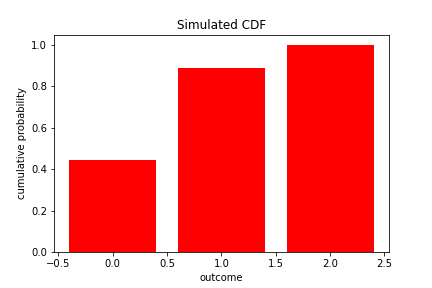
\includegraphics[width=8cm]{simulated CDF.png}
    \caption{simulated CDF}
\end{figure}
\begin{figure}[h!]
    \centering
    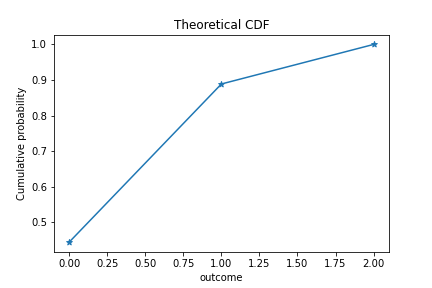
\includegraphics[width=8.25cm]{Theoretical CDF.png} 
    \caption{Theoretical CDF}
\end{figure}
\begin{figure}[h!]
    \centering
    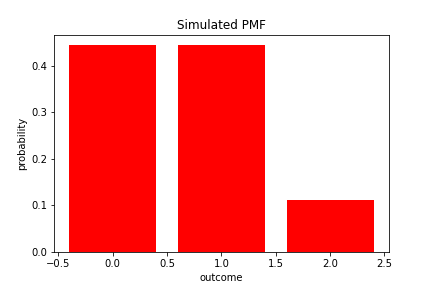
\includegraphics[width=8.25cm]{simulated PMF.png} 
    \caption{simulated PMF}
\end{figure}
\begin{figure}[h!]
    \centering
    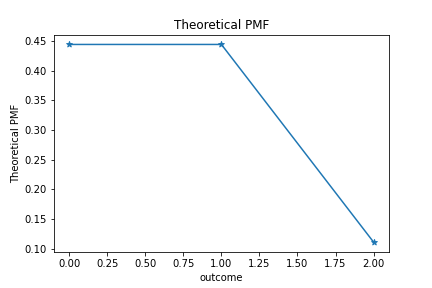
\includegraphics[width=8.25cm]{Theoretical PMF.png}
    \caption{theoretical PMF}
\end{figure}
\section{six appear on at-least one die}
since a pair of dies are thrown,\\
There can be two cases
\begin{enumerate}
    \item six does not appear at all
    \item six appear on atleast one die
\end{enumerate}
Hence,\\ Z=0 six does not appears at all\\
Z=1 appears on atleast die
\\ \textbf{Finding P(Z=1)}\\
ie,probability that at-least one six appears
\begin{align*}
P(Z=1)&=P(X=6)\&P(Y<6)+P(X<6)\&P(Z=6)\\
&\quad +P(X=6)\&P(Y=6)\\
&=\frac{1}{6}\times\frac{5}{6}+\frac{5}{6}\times\frac{1}{6}+\frac{1}{6}\times\frac{1}{6}\\
&=\frac{11}{36}
\end{align*}

\textbf{Finding P(Z=0)}
\\i.e,probability that six does-not appear
\begin{align*}
\hspace{-3cm}
    P(Z=0)&=P(X<6)\&P(Y<6)\\
    &=\frac{5}{6}\times\frac{5}{6}\\
    &=\frac{25}{36}
\end{align*}
Therefore,P(X=0)=$\frac{25}{36}$
so,our probability distribution is
\begin{table}[ht]
    \centering
    \begin{tabular}{|c|c|c|}
    \hline
         X&0&1\\[5pt]
         \hline
         P(X)&$\frac{25}{36}$&$\frac{11}{36}$\\[5pt]
         \hline
    \end{tabular}
    \caption{probability distribution}
    \label{tab:my_label}
\end{table}
\begin{figure}[h!]
    \centering
    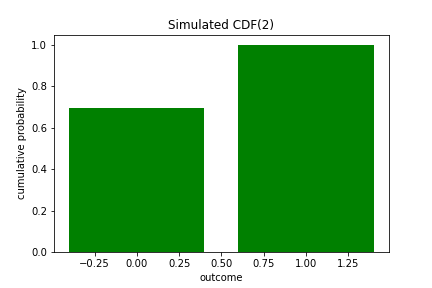
\includegraphics[width=9cm]{simulated CDF(2).png}
    \caption{simulated CDF}
\end{figure}
\begin{figure}[h!]
    \centering
    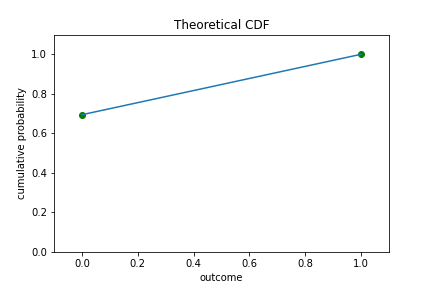
\includegraphics[width=9cm]{Theoretical CDF(2).png} 
    \caption{Theoretical CDF}
\end{figure}
\begin{figure}[h!]
    \centering
    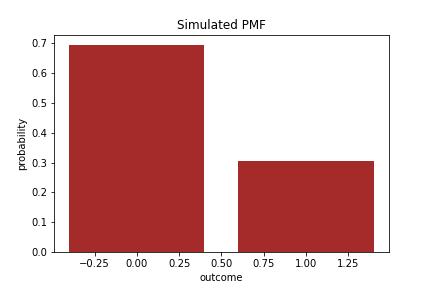
\includegraphics[width=9cm]{simulated PMF(2).png} 
    \caption{simulated PMF}
\end{figure}
\begin{figure}[h!]
    \centering
    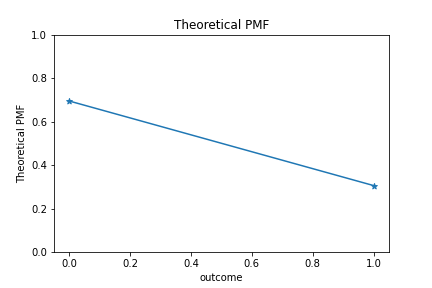
\includegraphics[width=9cm]{Theoretical PMF(2).png}
    \caption{theoretical PMF}
\end{figure}
\end{document}
